\documentclass[border={0.1cm 0.1cm 0.1cm 0.1cm}]{standalone}  %E,S,W,N

\usepackage{amssymb}
\usepackage{amsmath}
\usepackage{tikz}
\usetikzlibrary{shapes} 				%for node shapes
\usetikzlibrary{calc}					%for centerarc
\usetikzlibrary{arrows, arrows.meta}	%for big arrowheads

\def\centerarc[#1](#2)(#3:#4:#5) {\draw[#1] ($(#2)+({#5*cos(#3)},{#5*sin(#3)})$) arc (#3:#4:#5);}

\newcommand\irregularline[2]{%
	let \n1 = {rand*(#1)} in +(0,0*\n1)
	\foreach \a in {0.1,0.2,...,#2}{let \n1 = {rand*(#1)} in --+(\a,\n1)} }

%by Brenton Ables, based on his Ph.D thesis: A Deleuzian Theory of Eternity
%https://atrium.lib.uoguelph.ca/xmlui/handle/10214/14775

\begin{document}
	
	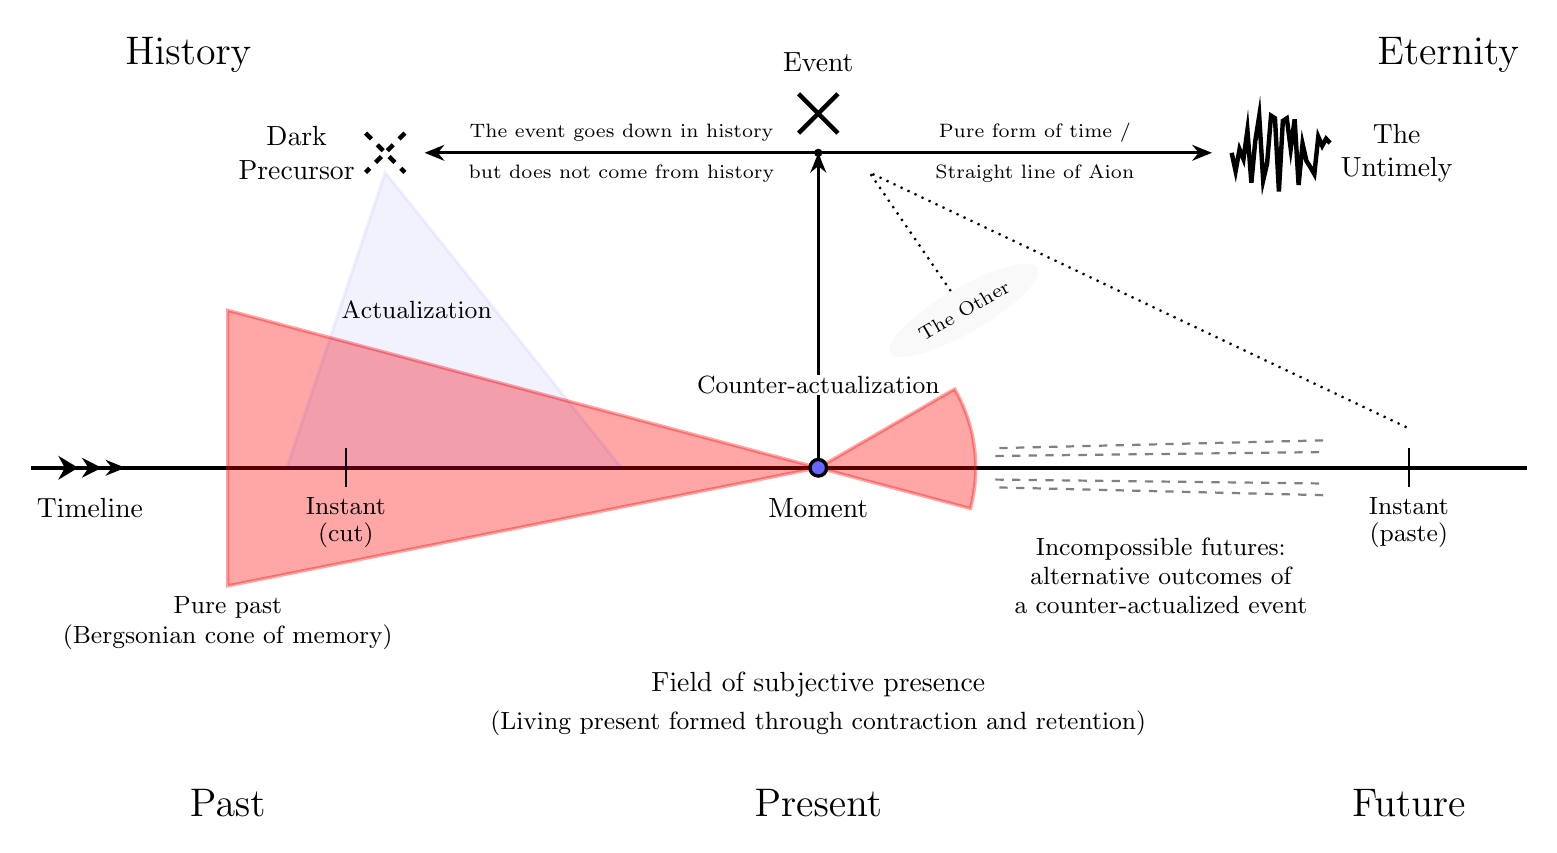
\begin{tikzpicture}[very thick]	
	%MAIN AXIS
	\draw[ultra thick] (-10,0)--(9,0);
	
	%THE OTHER
	\draw[thick,dotted] (1.85,2)--(0.65,3.75)--(7.5,0.5);
	\node[ellipse,rotate=30,fill=gray!5,semithick] at (1.85,2) {\scriptsize The Other};
	
	%CENTRAL CIRCLE
	\centerarc[-{Stealth[length=2.5mm,width=2mm]}](0,0)(0:45:2)
	\centerarc[-{Stealth[length=2.5mm,width=2mm]}](0,0)(45-3:45+25:2)
	\centerarc[-{Stealth[length=2.5mm,width=2mm]}](0,0)(0:-45:2)
	\centerarc[-{Stealth[length=2.5mm,width=2mm]}](0,0)(-42:-45-25:2)
	%
	\centerarc[-{Stealth[length=2.5mm,width=2mm]}](0,0)(180:180-45:2)
	\centerarc[-{Stealth[length=2.5mm,width=2mm]}](0,0)(180-45:180-45-25:2)
	\centerarc[-{Stealth[length=2.5mm,width=2mm]}](0,0)(180:180+45:2)
	\centerarc[-{Stealth[length=2.5mm,width=2mm]}](0,0)(180+45:180+45+25:2)
	%
	\centerarc[](0,0)(69:136:2)
	\centerarc[](0,0)(224:301:2)
	
	%UPPER PART
	\draw[-{Stealth[length=2.5mm,width=2mm]}] (0,0)--(0,4);
	\fill (0,4) circle (1.5pt);
	\draw[{Stealth[length=2.5mm,width=2mm]}-{Stealth[length=2.5mm,width=2mm]}] (-5,4)--(5,4);
	\draw[ultra thick] (0-0.25,4.5+0.25)--(0+0.25,4.5-0.25); %X
	\draw[ultra thick] (0+0.25,4.5+0.25)--(0-0.25,4.5-0.25); %X
	\node at (0,5.15) {Event};
	%
	\draw[ultra thick,dashed] (-5.5-0.25,4+0.25)--(-5.5+0.25,4-0.25); %X (dark precursor)
	\draw[ultra thick,dashed] (-5.5+0.25,4+0.25)--(-5.5-0.25,4-0.25); %X (dark precursor)
	\node[align=center,left] at (-5.75,4) {Dark \\ Precursor};
	%
	\node[align=center] at (-2.5,4) {%
		\scriptsize The event goes down in history \\[1mm]
		\scriptsize but does not come from history
	};
	\node[align=center] at (2.75,4) {%
		\scriptsize Pure form of time / \\[1mm]
		\scriptsize Straight line of Aion
	};
	
	%THE UNTIMELY
	\draw[ultra thick,xscale=0.5,yshift=-0.5cm] (2*5.25,4.5) \irregularline{0.5cm}{2.5};
	\node[align=center,right] at (6.5,4) {The \\ Untimely};
	
	%TRIANGLES
	\filldraw[fill=red,draw=red,opacity=.35] (0,0)--({2*cos(-15)},{2*sin(-15)}) arc (-15:30:2cm)--cycle;
	\filldraw[fill=red,draw=red,opacity=.35] (0,0)--(-7.5,2)--(-7.5,-1.5)--cycle;
	\draw[semithick] (-6,0.25)--(-6,-0.25) node[below,align=center] {%
		\small Instant \\[-0.75mm] \small (cut)};
	\node[below,align=center] at (-7.5,-1.5) {%
		\small Pure past \\[-0.5mm]
		\small (Bergsonian cone of memory)
	};
	\filldraw[fill=blue,draw=blue,opacity=0.05] (-6.75,0)--(-5.5,3.75)--(-2.5,0)--cycle;
	\node at (-5.1,2) {\small Actualization};
	
	%LOWER LABELS
	\filldraw[fill=blue!60] (0,0) circle (3pt);
	\node[below,yshift=-0.25cm] at (0,0) {Moment};
	\node[fill=white,inner sep=0.5] at (0,1.05) {\small Counter-actualization};
	\node[align=center] at (0,-3) {%
		Field of subjective presence \\[0.5mm]
		\small (Living present formed through contraction and retention)		
	};
	\node at (-7.5,-4.25) {\Large Past};		\node at (-8,5.25) {\Large History};
	\node at (0,-4.25) {\Large Present};
	\node at (7.5,-4.25) {\Large Future};	\node at (8,5.25) {\Large Eternity};
	%
	\draw[semithick] (7.5,0.25)--(7.5,-0.25) node[below,align=center] {\small Instant \\[-0.75mm] \small (paste)};
	\draw[thick,gray,dashed] (2.25,0.15)--++(4.2,0.05);
	\draw[thick,gray,dashed] (2.25,-0.15)--++(4.2,-0.05);
	\draw[thick,gray,dashed] (2.3,0.25)--++(4.2,0.1);
	\draw[thick,gray,dashed] (2.3,-0.25)--++(4.2,-0.1);
	%
	\node[below,align=center] at (4.35,-0.75) {%
		\small Incompossible futures: \\[-0.5mm]
		\small alternative outcomes of \\[-0.5mm]
		\small a counter-actualized event
	};
	%
	\draw[-{Stealth[length=2.5mm,width=3mm]}] (-10,0)--(-9.4,0);
	\draw[-{Stealth[length=2.5mm,width=2.5mm]}] (-9.4,0)--(-9.1,0);
	\draw[-{Stealth[length=2.5mm,width=2mm]}] (-9.1,0)--(-8.8,0);
	\node[below,yshift=-0.25cm] at (-9.25,0) {Timeline};
	\end{tikzpicture}
	
\end{document}